\documentclass[8pt,landscape]{article}

% PACKAGES
\usepackage[letterpaper, margin=0.25in]{geometry} % tighter margins
\usepackage{amsmath, amssymb}
\usepackage{multicol}
\usepackage{setspace}
\usepackage{sectsty}
\usepackage{verbatim}
\usepackage{graphicx}
% --- FORMATTING ---
\setstretch{0.9}
\setlength{\parindent}{0pt}
\setlength{\parskip}{0pt}
\allsectionsfont{\fontsize{8}{8}\selectfont}
% Reduce subsection spacing
\makeatletter
\renewcommand{\subsection}{\@startsection{subsection}{2}{0pt}%
    {0.2ex}% space before subsection
    {0.2ex}% space after subsection
    {\fontsize{8}{8}\bfseries}} % font size and bold
\makeatother
% DOCUMENT START
\begin{document}
\pagestyle{empty}
\begin{multicols}{3}

\subsection*{Discrete Distribution Families}

\subsection*{Binomial($n,p$)*binom} 
successes in $n$ Bernoulli trials. \\
PMF: $P(X=x)=\binom{n}{x}p^x(1-p)^{n-x}$ \\
Mean: $np$, Var: $np(1-p)$ 

\subsection*{Geometric($p$)*geom} 
Failures before 1st success. \\
PMF: $P(X=x)=(1-p)^x p$, $x \ge 0$ \\
Mean: $(1-p)/p$, Var: $(1-p)/p^2$ 

\subsection*{NegBin($k,p$)*nbinom} 
Failures before $k$-th success. \\
PMF: $P(X=x)=\binom{x+k-1}{x}p^k(1-p)^x$ \\
Mean: $k(1-p)/p$, Var: $k(1-p)/p^2$ 

\subsection*{Poisson($\lambda$)*pois}
Counts in interval, rate $\lambda$. \\
PMF: $P(X=x)=\tfrac{\lambda^x e^{-\lambda}}{x!}$ \\
Mean: $\lambda$, Var: $\lambda$ 

\subsection*{Continuous Distribution Families}

\subsection*{Uniform($a,b$) - *unif} 
All values equally likely on $[a,b]$. \\
PDF: $f(x)=\tfrac{1}{b-a}, \; a \le x \le b$ \\
Mean: $(a+b)/2$, Var: $(b-a)^2/12$ 

\subsection*{Normal($\mu,\sigma^2$) - *norm}
Bell-shaped, $-\infty < \mu < \infty , \sigma^2 > 0 $\\
PDF: $f(x)=\tfrac{1}{\sqrt{2\pi\sigma^2}} e^{-(x-\mu)^2/(2\sigma^2)}$ \\
Mean: $\mu$, Var: $\sigma^2$ \\
Z score: $\mu = x - Z\sigma$ 

\subsection*{Lognormal($\mu,\sigma^2$) - *lnorm}
If $\ln X \sim N(\mu,\sigma^2)$. \\
PDF: $f(x)=\tfrac{1}{x\sigma\sqrt{2\pi}} e^{-(\ln x-\mu)^2/(2\sigma^2)}$ \\
Mean: $e^{\mu+\sigma^2/2}$, Var: $(e^{\sigma^2}-1)e^{2\mu+\sigma^2}$ \\
Skewness: $(e^{\sigma^2}+2)\sqrt{e^{\sigma^2}-1}$ 

\subsection*{Exponential($\lambda$) - *exp}
Time between Poisson events, Positive RV, wait time, memoryless \\
($\lambda$) is average rate ($\beta$) is mean wait time \\
PDF: $f(x)=\lambda e^{-\lambda x}, x\ge0$ \\
Mean: $1/\lambda$, Var: $1/\lambda^2$ \\
Skewness: 2 

\subsection*{Beta($\alpha,\beta$) - *beta}
On $[0,1]$, Bayesian priors. Uniform distribution special case \\
($\Gamma$) function is a generalization of factorial function to non-integer numbers. \\
PDF: $f(x)=\tfrac{1}{B(\alpha,\beta)} x^{\alpha-1}(1-x)^{\beta-1}$ \\
Mean: $\alpha/(\alpha+\beta)$, Var: $\tfrac{\alpha\beta}{(\alpha+\beta)^2(\alpha+\beta+1)}$ \\
Skewness: $\frac{2(\beta-\alpha)\sqrt{\alpha+\beta+1}}{(\alpha+\beta+2)\sqrt{\alpha\beta}}$ 

\subsection*{Weibull($k,\lambda$) - *weibul}
Lifetimes, survival, reliability. \\
Exponential family (when k = 1), longer you wait \\
Survival Analysis \\
PDF: $f(x)=\tfrac{k}{\lambda}(x/\lambda)^{k-1} e^{-(x/\lambda)^k}$ \\
Mean: $\lambda \Gamma(1+1/k)$, Var: $\lambda^2[\Gamma(1+2/k)-\Gamma(1+1/k)^2]$ \\
Skewness: $\frac{\Gamma(1+3/k)\lambda^3 - 3\mu\sigma^2 - \mu^3}{\sigma^3}$ 

\subsection*{Continuous RV (numerical integration)}
\texttt{f <- function(x) 2*x} \\
\texttt{EV <- integrate(function(x) x*f(x), 0,1)\$value} \\
\subsection*{Define the PDF function}
\texttt{f <- function(x) { 2*x }} \\
\texttt{prob <- integrate(f, lower = 0.5, upper = 0.75)\$value \# Integrate over [0.5, 0.75]}
\subsection*{Conditional Distributions}
\texttt{Conditional dist is just a segment of marginal dist, then re-normalized to have an area under the curve equal to 1}
\texttt{If X and Y are independent, in continouse case,\[
f_{Y|X}(y) = f_Y(y)\] This means conditional PDF of Y and X is marginal PDF of Y. }
\subsection*{Random Sample}
\texttt{It is independent and identically distributed (iid). Each pair of observations are independent, and each observation comes from the same distribution.}
\subsection*{MLE}
\texttt{Great way to find estimators. Applied on multi and univariate. Relies on random sample of n observations. Mean, is a estimator for univariate, multivariate, linear regression}
\subsection*{Steps for MLE}
\texttt{1.(discrete or contin) distribution} \\
\texttt{2.Find parameters of a theoretical distribution (eg $\lambda$ in a Poisson distribution)} \\
\texttt{3.Choose distribution)} \\
\texttt{4.Play with the parameters for that family of distributions to find the most likely parameters for the corresponding parametric estimates)} \\
\texttt{5.To get estimates, we use the likelihood function of our observed random sample.)} \\
\subsection*{Joint PDF and Likelihood Function}
The Joint PDF and Likelihood function is defined as:
\[
f(x_1, x_2, \dots, x_n;\theta) = L(\theta \mid x_1, x_2, \dots, x_n) = \prod_{i=1}^n f(x_i;\theta)
\]
\subsection*{R: Generating Sample and Likelihood}
\begin{verbatim}
#Generate 30 random samples from Exponential(beta=20)
set.seed(123)
sample_n30 <- tibble(values = rexp(30, rate = 1/20))
#Compute likelihood and log-likelihood for candidate
exp_values <- tibble(
  possible_betas = seq(5, 50, 0.5),
  likelihood = map_dbl(1 / possible_betas, 
   ~ prod(dexp(sample_n30$values, .))),
  log_likelihood = map_dbl(1 / possible_betas, 
   ~  log(prod(dexp(sample_n30$values, .))))
)
empirical_MLE <- exp_values |>
  arrange(desc(likelihood)) |>
  slice(1)
analytical_MLE <- mean(sample_n30$values) 
#We use the sample mean() function from R!
round(analytical_MLE, 2)
LL <- function(l) log(prod(dexp(sample_n30$values,
rate = 1 / l)))
optimize(LL, c(5, 50), maximum = TRUE)
stochastic - having some uncertain outcome. 
deterministic - an outcome that will be known 
with 100% certainty.
Computers cannot actually generate truly 
random outcomes. 
Instead, they use something called 
pseudorandom numbers.
Although this sequence is deterministic, 
it behaves like a random sample. 
One pitfall is that neighbouring pairs are not 
independent of each other.

The empirical approach (using observed data),
resulting in approximate values that improve 
as the sample size increases 
(i.e., the frequentist paradigm!).

The Law of Large of Numbers states that, as we 
increase our sample size n, our empirical mean 
converges to the true mean we want to estimate.
\end{verbatim}
\subsection*{Skewness}
\begin{center}
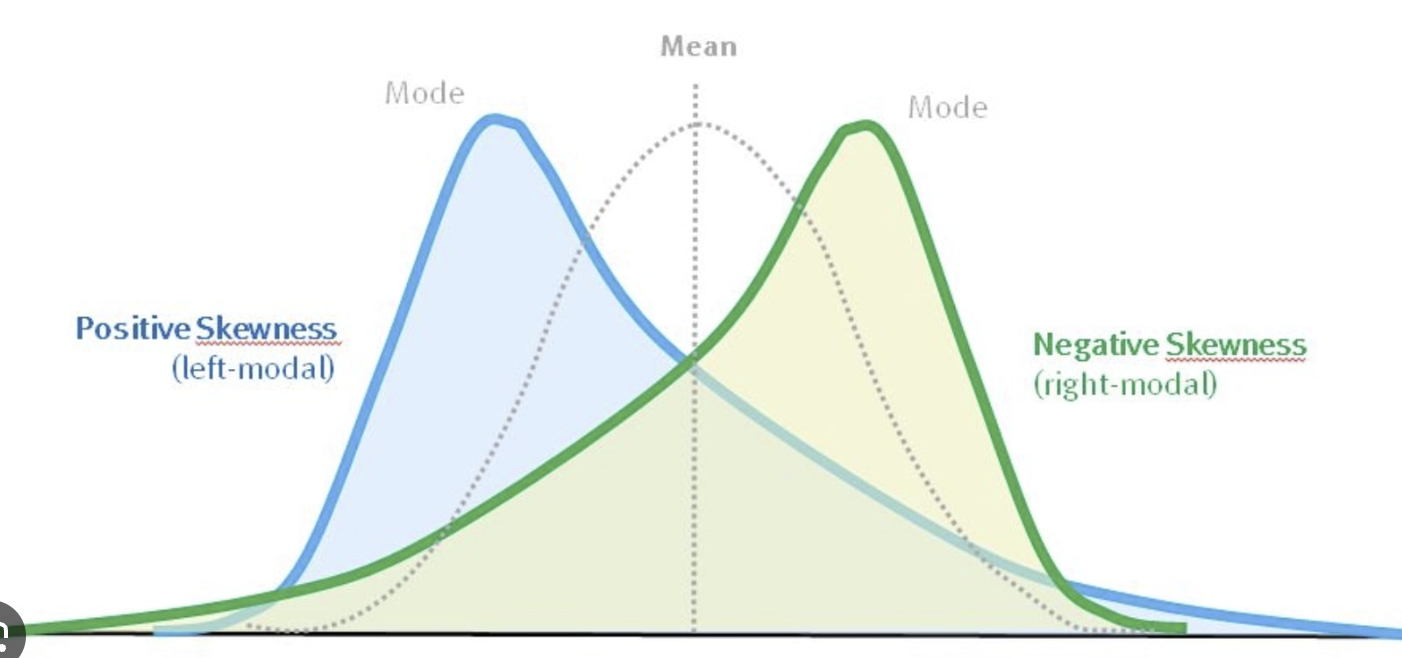
\includegraphics[width=0.9\linewidth]{skew.png}
\end{center}
\texttt{Left-skewed: long tail to the left, mean < median < mode} \\
\texttt{Right-skewed: long tail to the right, mean > median > mode} \\
\end{multicols}
\end{document}